
\documentclass[12pt]{article}
 
\usepackage[margin=1in]{geometry} 
\usepackage{amsmath,amsthm,amssymb,scrextend}
\usepackage{fancyhdr}
\pagestyle{fancy}
\DeclareMathOperator{\rng}{Rng}
\DeclareMathOperator{\dom}{Dom}
\newcommand{\R}{\mathbb R}
\newcommand{\cont}{\subseteq}
\newcommand{\N}{\mathbb N}
\newcommand{\Z}{\mathbb Z}
\usepackage{tikz}
\usepackage{pgfplots}
\usepackage{amsmath}
\usepackage[mathscr]{euscript}
\let\euscr\mathscr \let\mathscr\relax% just so we can load this and rsfs
\usepackage[scr]{rsfso}
\usepackage{amsthm}
\usepackage{amssymb}
\usepackage{multicol}
\usepackage{mathtools}
%\usepackage{ngerman}
\usepackage[colorlinks=true, pdfstartview=FitV, linkcolor=blue,
citecolor=blue, urlcolor=blue]{hyperref}

\DeclareMathOperator{\arcsec}{arcsec}
\DeclareMathOperator{\arccot}{arccot}
\DeclareMathOperator{\arccsc}{arccsc}
\newcommand{\ddx}{\frac{d}{dx}}
\newcommand{\dfdx}{\frac{df}{dx}}
\newcommand{\ddxp}[1]{\frac{d}{dx}\left( #1 \right)}
\newcommand{\dydx}{\frac{dy}{dx}}
\let\ds\displaystyle
\newcommand{\intx}[1]{\int #1 \, dx}
\newcommand{\intt}[1]{\int #1 \, dt}
\newcommand{\defint}[3]{\int_{#1}^{#2} #3 \, dx}
\newcommand{\imp}{\Rightarrow}
\newcommand{\un}{\cup}
\newcommand{\inter}{\cap}
\newcommand{\ps}{\mathscr{P}}
\newcommand{\set}[1]{\left\{ #1 \right\}}
\newtheorem*{sol}{Solution}
\newtheorem*{claim}{Claim}
\newtheorem{problem}{Problem}

\newcommand\parttwo{\stackrel{\mathclap{\normalfont\mbox{2}}}{=}}
\newcommand\partthree{\stackrel{\mathclap{\normalfont\mbox{3}}}{=}}
\newcommand\partsix{\stackrel{\mathclap{\normalfont\mbox{6}}}{=}}
\newcommand\partseven{\stackrel{\mathclap{\normalfont\mbox{7}}}{=}}
\begin{document}
 

\lhead{Formal Logic Sheet 11}
\chead{Robert Feldhans, Sebastian Mueller}
\rhead{\today}


\section*{Exercise 41: (Relations and directed graphs)}

See Figure below

\begin{figure}[ht]
	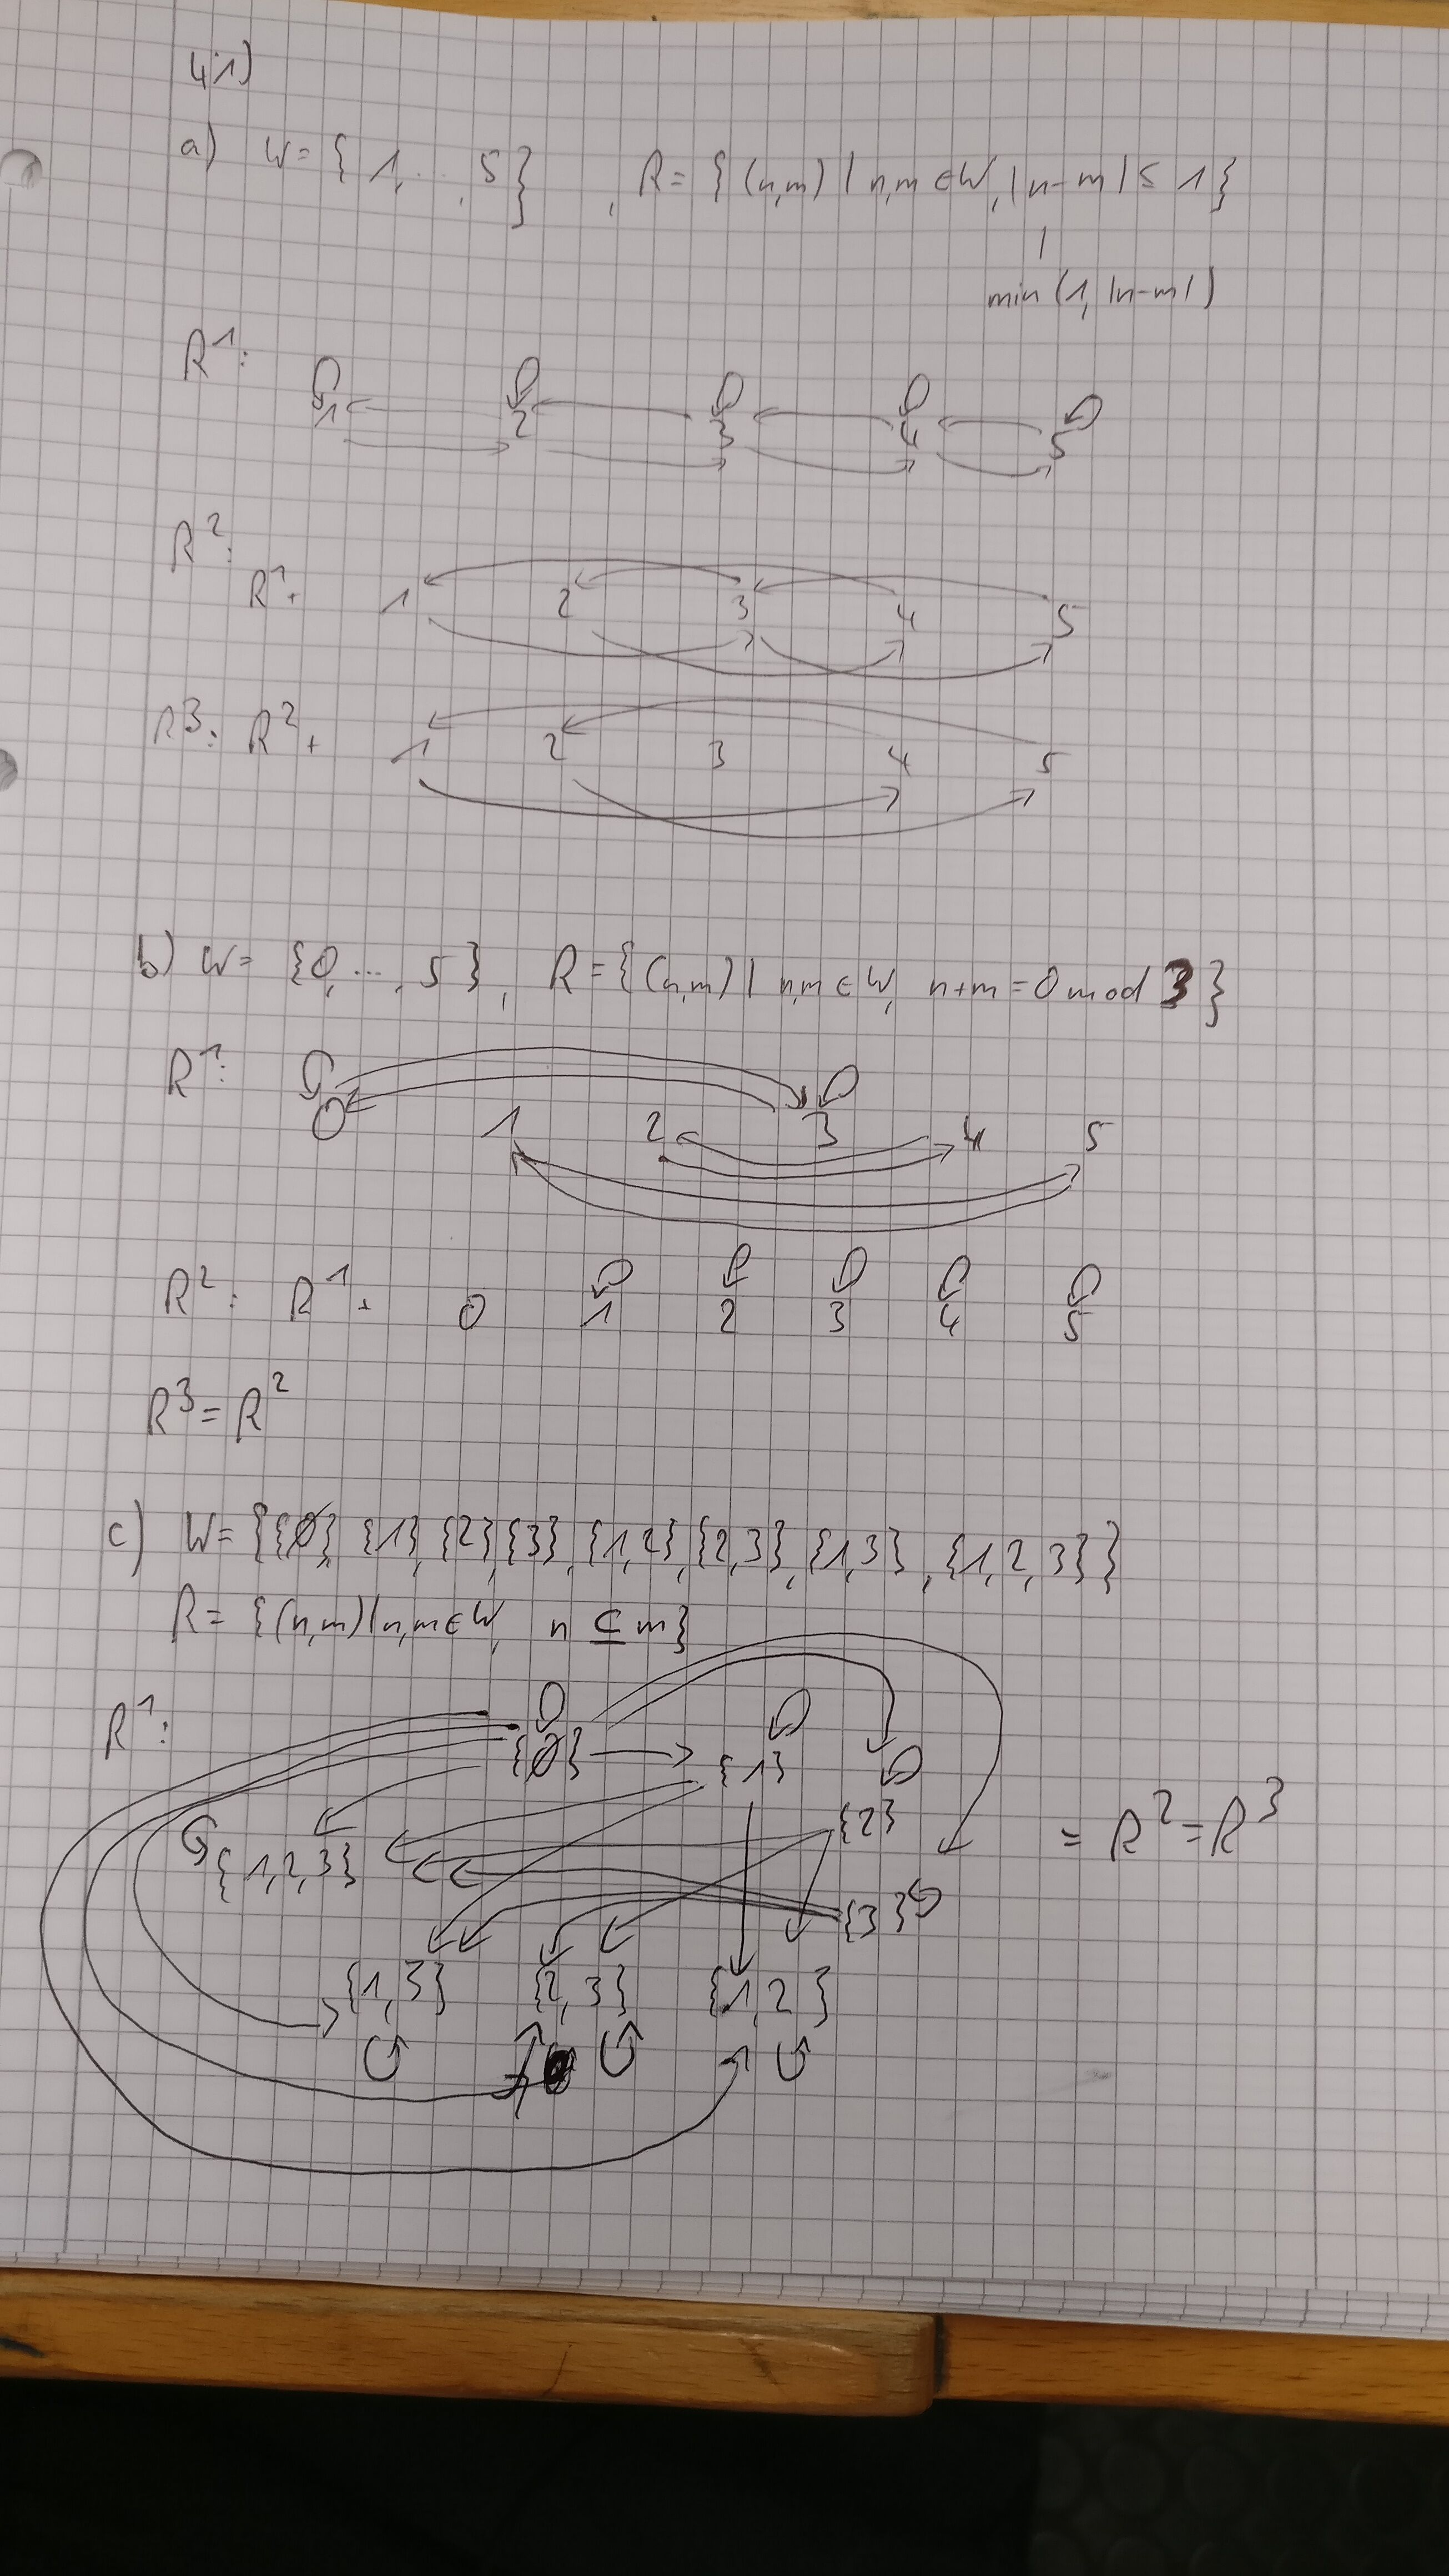
\includegraphics[scale=0.1475]{../pics/41.jpeg}
	\caption{Solution for Exercise 41}
\end{figure}

\section*{Exercise 42: (Rules)}

See Figure below

\begin{figure}[ht]
	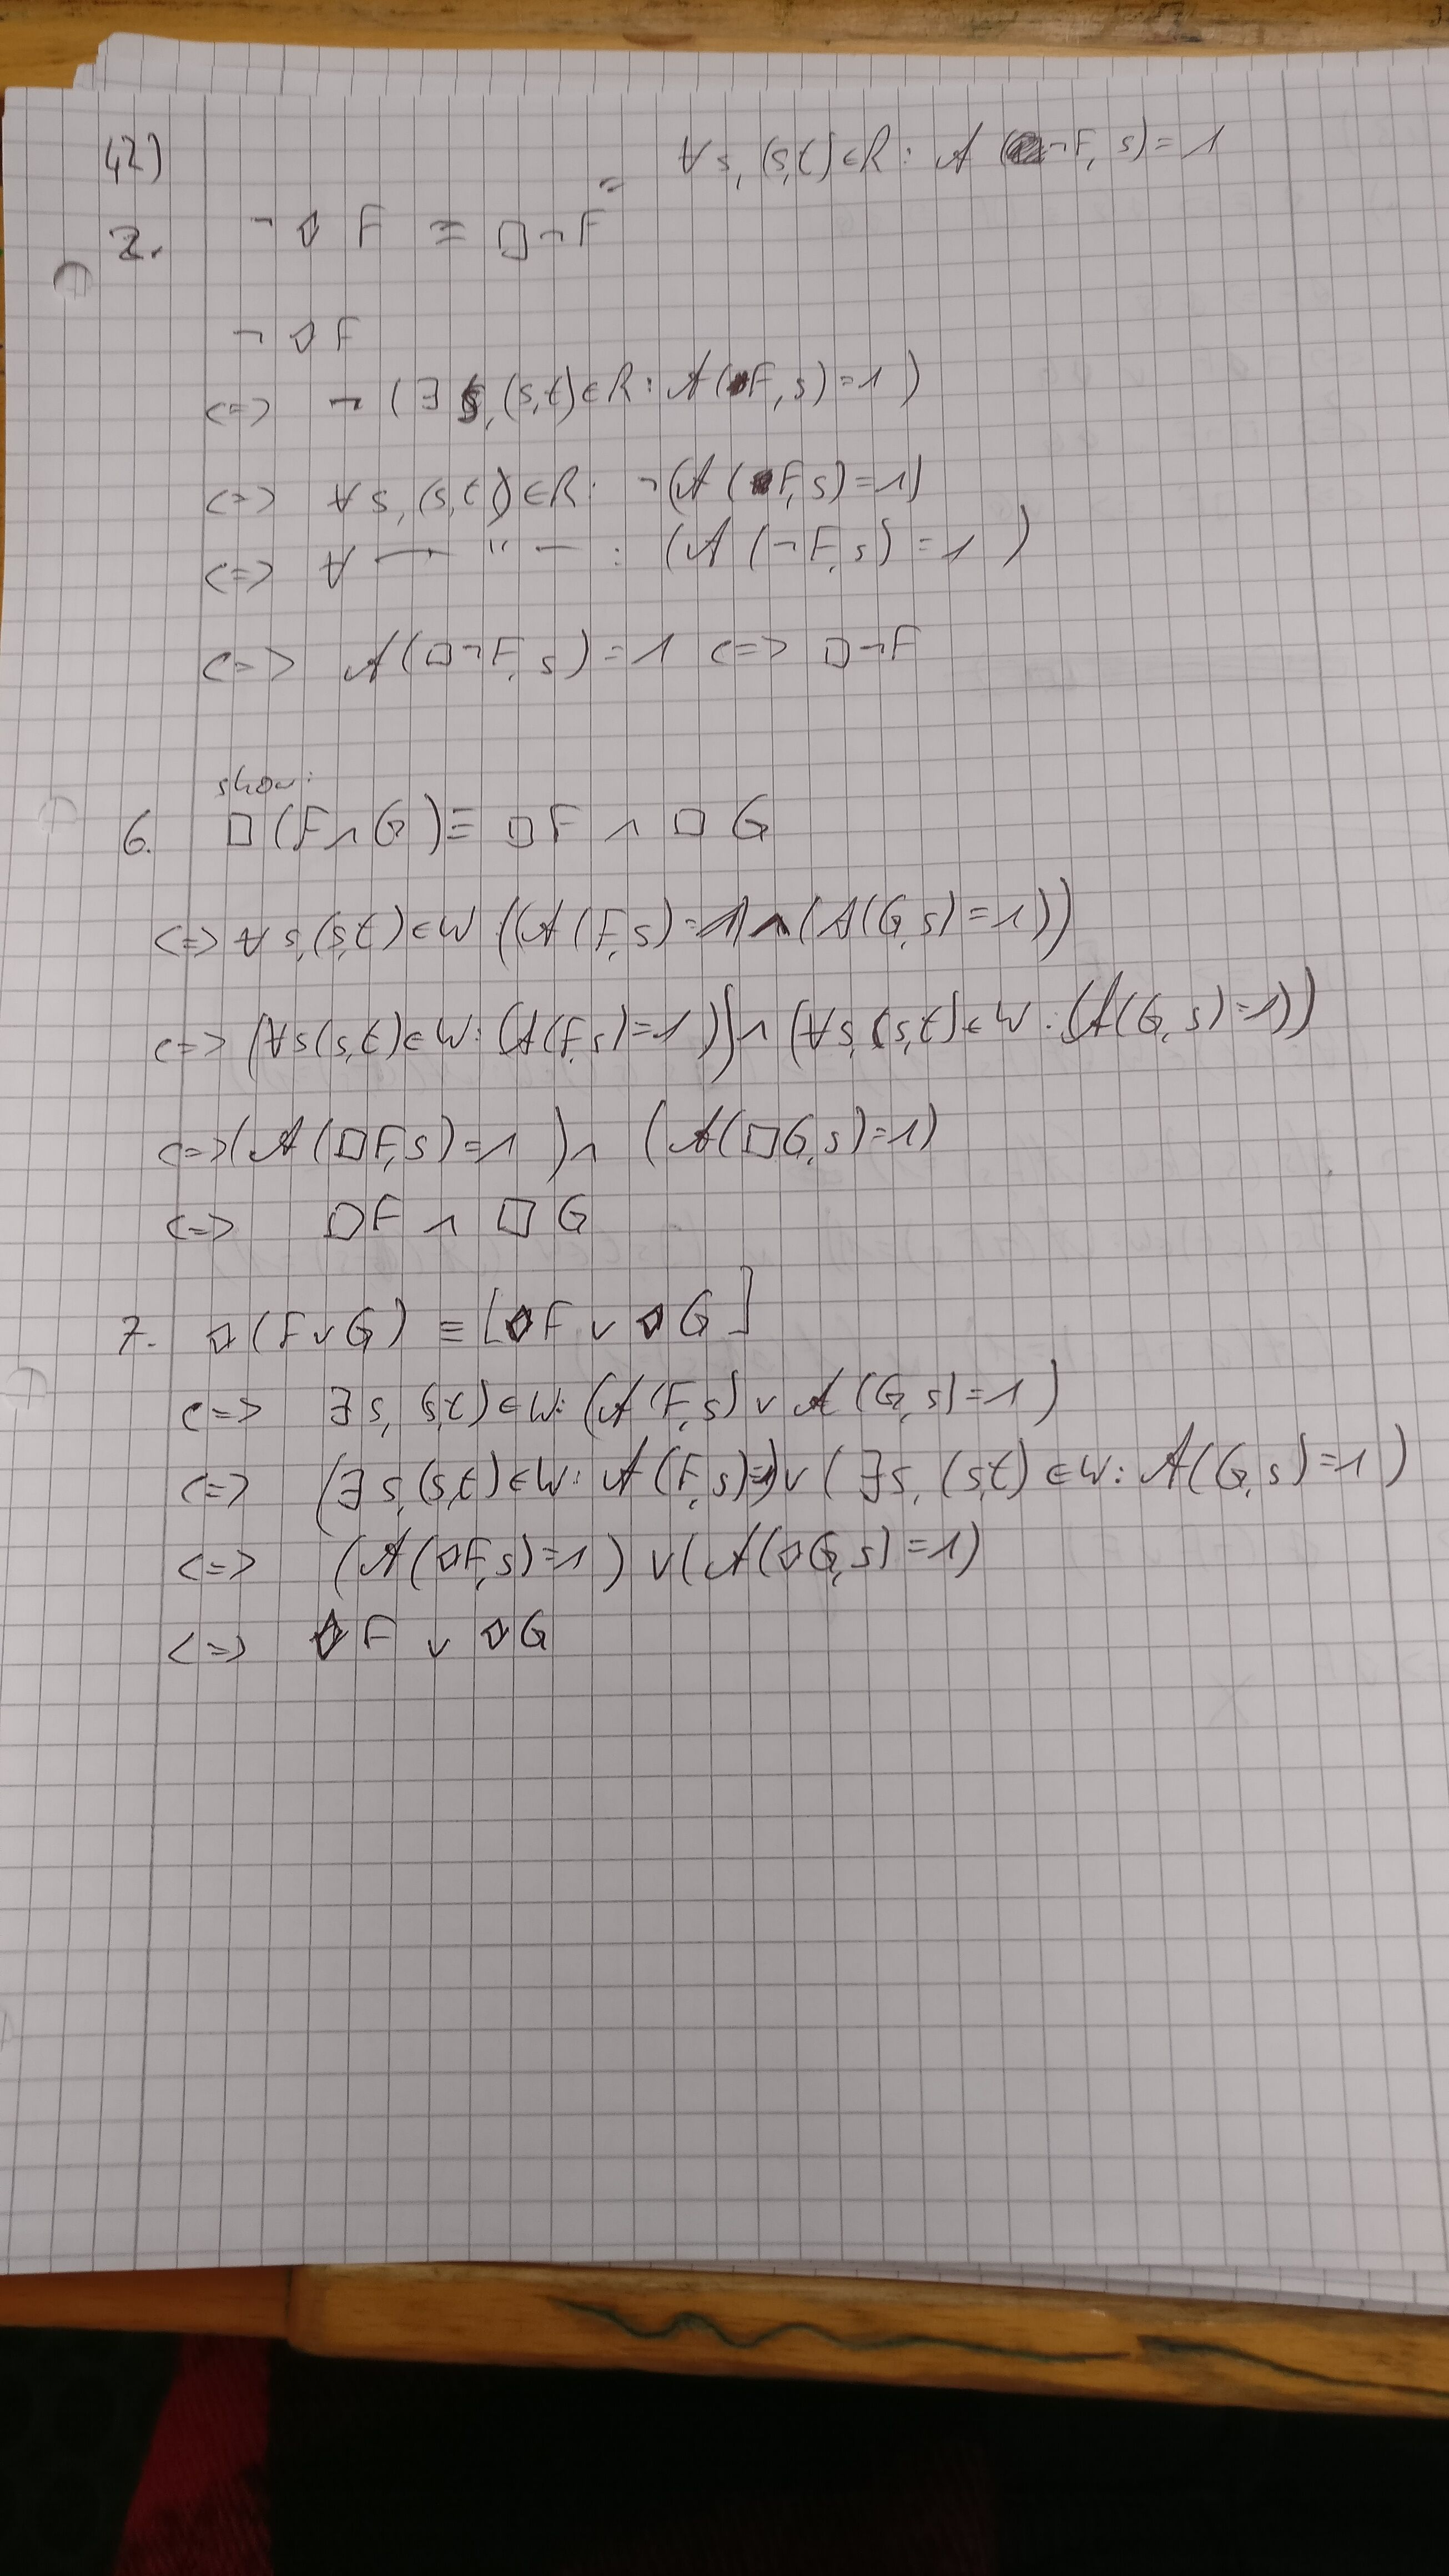
\includegraphics[scale=0.1475]{../pics/42.jpeg}
	\caption{Solution for Exercise 42}
\end{figure}

\section*{Exercise 43: (More rules)}

See Figure below

\begin{figure}[ht]
	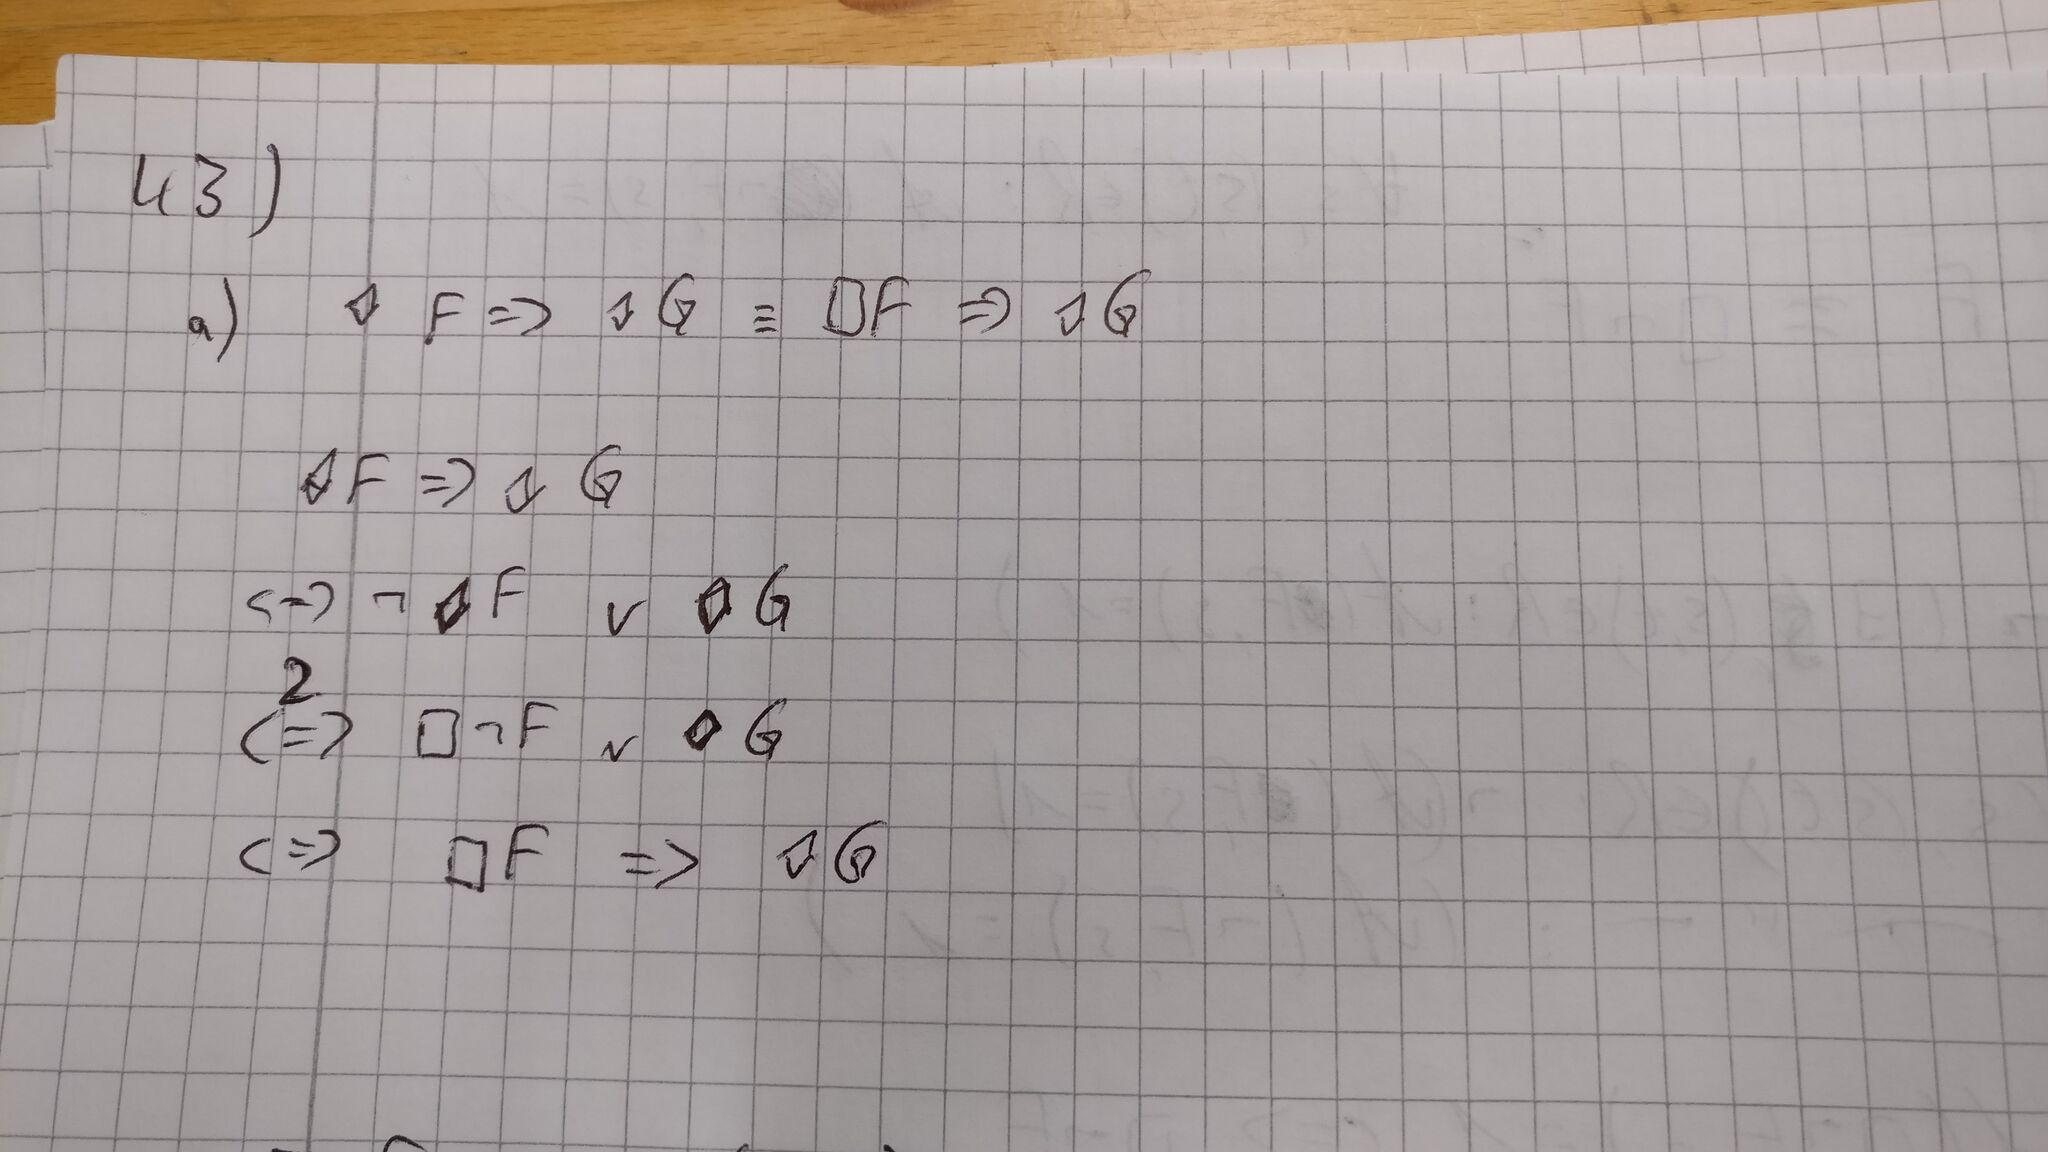
\includegraphics[scale=0.25]{../pics/43a.jpeg}
	\caption{Solution for Exercise 43}
\end{figure}

\section*{Exercise 44: (Tautologies)}

\subsection*{a}
$\square F \Rightarrow \diamond F$\\\\
$(\forall s,(s,t)\in W:(A(F,s)=1)) \Rightarrow (\exists s,(s,t) W:(A(F,s)=1))$\\\\
$\lnot (\forall s,(s,t)\in W:(A(F,s)=1)) \lor (\exists s,(s,t) W:(A(F,s)=1)) $\\\\
$ (\exists s,(s,t)\in W:(A(\lnot F,s)=1)) \lor (\exists (s,t) W:(A(F,s)=1)) $\\\\
$(A(\diamond \lnot F, s)=1) \lor (A(\diamond F,s)=1)$\\\\
$\diamond \lnot F \lor \diamond F$\\\\
$\partseven \diamond (F \lor \lnot F) $\\
Is a tauntology.

\subsection*{b}
$F \Rightarrow \diamond F$\\

\subsection*{c}
$\square F \Leftrightarrow \lnot \diamond \lnot F$\\\\
$\parttwo \square F \Leftrightarrow \lnot \lnot \square F $\\
Is a tauntology.

\subsection*{d}
$(\square F \land \square (F \Rightarrow G)) \Rightarrow \square G$\\\\
$\partsix \square (F \land (F \Rightarrow G)) \Rightarrow \square G$\\\\
$\partthree F \land (F \Rightarrow G) \Rightarrow G$\\
Is not a tauntology.

\subsection*{e}
$\lnot (\square (F \Rightarrow G) \land \diamond F \land \square \lnot G)$\\\\
$\partsix \lnot (\square ((F \Rightarrow G) \land \lnot G) \land \diamond F)$\\\\
$\parttwo \lnot (\square ((F \Rightarrow G) \land \lnot G) \land \lnot \square \lnot F)$\\\\
$\partsix \lnot (\square ((F \Rightarrow G) \land \lnot G \land F))$

%ANARCHY
\end{document}